\section{Техническое задание}
\subsection{Основание для разработки}

Основанием для разработки является задание на выпускную квалификационную работу бакалавра "<Разработка web-платформы для поиска работы">.

\subsection{Цель и назначение разработки}

Основной задачей выпускной квалификационной работы является разработка  web-платформы для поиска работы.

Задачами данной разработки являются:
\begin{itemize}
\item создание информационных разделов платформы;
\item реализация формы для создания резюме;
\item реализация формы для создания вакансий;
\item реализация функционала для отклика на вакансии и резюме;
\item создание удобного поиска по вакансиям и резюме.
\end{itemize}

\subsection{Требования пользователя к интерфейсу web-сайта}

Сайт должен включать в себя:
\begin{itemize}
    \item навигацию по разделам;
    \item авторизацию;
    \item доступы для пользователя, администратора;
    \item формы для создания вакансий и резюме;
    \item возможность откликнуться на вакансию и резюме.
\end{itemize}

%\vspace{-\figureaboveskip} % двойной отступ не нужен (можно использовать, если раздел заканчивается картинкой)

\subsection{Моделирование вариантов использования}

Для разрабатываемого сайта была реализована модель, которая обеспечивает наглядное представление вариантов использования сайта.

Она помогает в физической разработке и детальном анализе взаимосвязей объектов. При построении диаграммы вариантов использования применяется унифицированный язык визуального моделирования UML.

Диаграмма вариантов описывает функциональное назначение разрабатываемой системы. То есть это то, что система будет непосредственно делать в процессе своего функционирования. Она является исходным концептуальным представлением системы в процессе ее проектирования и разработки. Проектируемая система представляется в виде ряда прецедентов, предоставляемых системой актерам или сущностям, которые взаимодействуют с системой. Актером или действующим лицом является сущность, взаимодействующая с системой извне (например, человек, техническое устройство). Прецедент служит для описания набора действий, которые система предоставляет актеру.

На основании анализа предметной области в программе должны быть реализованы следующие прецеденты:
\begin{enumerate}
\item Просмотр информации о платформе.
\item Просмотр списка вакансий, размещённых работодателями.
\item Просмотр информации о резюме соискателей, включая подробные данные о навыках, опыте, образовании и других аспектах, которые могут быть представлены в структурированном виде.
\item Добавление, редактирование резюме и вакансий
\item Поиск по вакансиям и резюме.
\end{enumerate}

Программа имеет четыре группы пользователей с разными правами:
гость, соискатель, работодатель и администратор.

Гостю должны быть доступны следующие функции:

\begin{enumerate}
	\item Просмотр информации о платформе.
	\item Регистрация на платформе.
	\item Поиск вакансий.
\end{enumerate}

Прецеденты для гостя представлены на рисунке ~\ref{p1:image}.

\begin{figure}[H]
	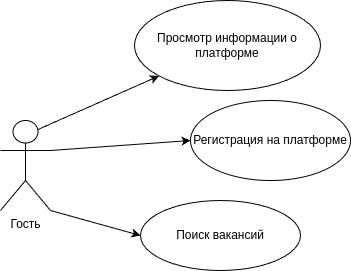
\includegraphics[width=0.7\linewidth]{p1}
	\caption{Диаграмма прецедентов для категории пользователей - гость}
	\label{p1:image}
\end{figure}

Соискателю должны быть доступны следующие функции:

\begin{enumerate}
	\item Авторизация на платформе.
	\item Создание и редактирование резюме.
	\item Поиск вакансий.
	\item Отклик на вакансию.
\end{enumerate}

Прецеденты для соискателя представлены на рисунке ~\ref{p2:image}.

\begin{figure}[H]
	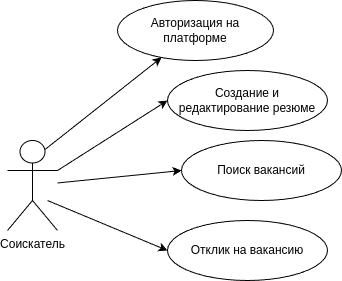
\includegraphics[width=0.7\linewidth]{p2}
	\caption{Диаграмма прецедентов для категории пользователей - соискатель}
	\label{p2:image}
\end{figure}

Работодателю должны быть доступны следующие функции:

\begin{enumerate}
	\item Авторизация на платформе.
	\item Публикация вакансии.
	\item Просмотр резюме соискателей.
	\item Просмотр откликов на вакансию.
\end{enumerate}

\begin{figure}[H]
	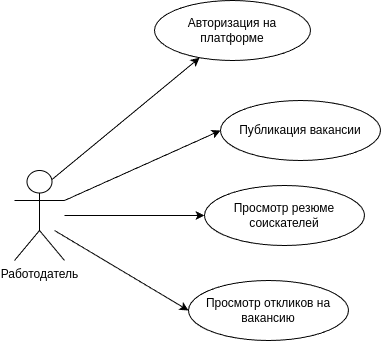
\includegraphics[width=0.7\linewidth]{p3}
	\caption{Диаграмма прецедентов для категории пользователей - работодатель}
	\label{p3:image}
\end{figure}

Aдминистратору должны быть доступны следующие функции:

\begin{enumerate}
	\item Управление пользователями.
	\item Модерация вакансий и резюме.
	\item Управление информационными разделами.
\end{enumerate}

\begin{figure}[H]
	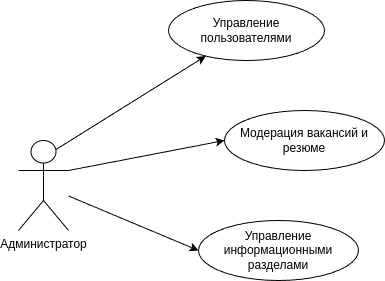
\includegraphics[width=0.7\linewidth]{p4}
	\caption{Диаграмма прецедентов для категории пользователей - администратор}
	\label{p4:image}
\end{figure}

\subsubsection{Вариант использования «Регистрация пользователя»}
Соискатель и работодатель желают зарегистрироваться на платформе для доступа к её функционалу (создание резюме/вакансий, поиск, отклики). Требуется простота процесса и безопасность данных.

Предусловие: пользователь открывает главную страницу платформы и нажимает кнопку «Зарегистрироваться».

Постусловие: пользователь успешно зарегистрирован, его данные сохранены в базе данных, и он перенаправлен в личный кабинет с подтверждением регистрации.

Основной успешный сценарий:

\begin{enumerate}
	\item Пользователь заполняет форму регистрации.
	\item Клиентская часть отправляет данные через HTTPS-запрос к REST API на сервер Symfony.
	\item Сервер проверяет уникальность email в базе данных MySQL.
	\item Если email уникален, сервер хеширует пароль с использованием алгоритма bcrypt и сохраняет данные пользователя в таблице users.
	\item Сервер генерирует токен JWT для авторизации и отправляет его клиенту.
	\item Клиент сохраняет токен в localStorage и перенаправляет пользователя в личный кабинет.
	\item Пользователь получает уведомление с ссылкой для подтверждения аккаунта.
\end{enumerate}

\subsubsection{Вариант использования «Создание резюме»}
Заинтересованные лица и их требования: соискатель хочет создать и опубликовать резюме для привлечения работодателей. Требуется удобный интерфейс и возможность редактирования данных.

Предусловие: пользователь авторизован как соискатель и находится в разделе «Моё резюме».

Постусловие: резюме создано, сохранено в базе данных и доступно для просмотра работодателями после модерации.

Основной успешный сценарий:

\begin{enumerate}
	\item Соискатель заполняет форму резюме в интерфейсе Vue.js.
	\item Клиент отправляет данные через API-запрос к серверу Symfony с токеном JWT.
	\item Сервер валидирует данные с использованием аннотаций Assert.
	\item Если данные валидны, сервер сохраняет резюме в таблице resumes через Doctrine и устанавливает статус «На модерации».
	\item Администратор (через панель управления) проверяет резюме и изменяет статус на «Опубликовано».
	\item Клиент сохраняет токен в localStorage и перенаправляет пользователя в личный кабинет.
	\item Соискатель получает уведомление об успешной публикации через email или интерфейс.
\end{enumerate}

\subsubsection{Вариант использования «Публикация вакансии»}
Заинтересованные лица и их требования: работодатель хочет опубликовать вакансию для привлечения соискателей. Требуется возможность указания детальных требований и модерации.

Предусловие: пользователь авторизован как работодатель и находится в разделе «Мои вакансии».

Постусловие: вакансия опубликована и доступна для просмотра соискателями после модерации.

Основной успешный сценарий:

\begin{enumerate}
	\item Работодатель заполняет форму вакансии в интерфейсе Vue.js.
	\item Клиент отправляет данные через API к серверу Symfony с токеном JWT.
	\item Сервер валидирует данные и сохраняет вакансию в таблице vacancies.
	\item Вакансия помечается как «На модерации», и администратор проверяет её на соответствие правилам.
	\item После одобрения статус меняется на «Опубликовано», и вакансия становится видимой в поиске.
	\item Работодатель получает уведомление о публикации.
\end{enumerate}

\subsubsection{Вариант использования «Поиск вакансий»}
Заинтересованные лица и их требования: соискатель хочет найти подходящие вакансии с помощью фильтров. Требуется быстрая и точная выдача результатов.

Предусловие: пользователь авторизован и находится на странице поиска вакансий.

Постусловие: список вакансий обновлён и отображает результаты, соответствующие выбранным фильтрам.

Основной успешный сценарий:

\begin{enumerate}
	\item Соискатель выбирает фильтры в интерфейсе Vue.js.
	\item Клиент отправляет запрос с параметрами фильтрации к API Symfony.
	\item Сервер выполняет SQL-запрос к таблице vacancies.
	\item Результаты сортируются по релевантности и возвращаются клиенту в формате JSON.
	\item Vue.js рендерит обновлённый список вакансий на странице.
	\item Соискатель просматривает результаты и может сохранить интересные вакансии в избранное.
\end{enumerate}

\subsubsection{Вариант использования «Отправка отклика»}
Заинтересованные лица и их требования: соискатель хочет подать отклик на вакансию, а работодатель — получить уведомление об отклике. Требуется простота процесса и уведомления.

Предусловие: соискатель авторизован, выбрал вакансию и нажал кнопку «Откликнуться».

Постусловие: отклик сохранён в базе данных, работодатель уведомлён, а соискатель получил подтверждение.

Основной успешный сценарий:

\begin{enumerate}
	\item Соискатель выбирает вакансию и нажимает «Откликнуться» в интерфейсе Vue.js.
	\item Клиент отправляет запрос к API Symfony с указанием.
	\item Сервер проверяет авторизацию и соответствие данных.
	\item Если данные корректны, сервер сохраняет отклик в таблице responses и генерирует уведомление.
	\item Уведомление отправляется работодателю через email и отображается в его личном кабинете.
	\item Соискатель получает подтверждение об успешной отправке отклика.
\end{enumerate}

\subsection{Требования к оформлению документации}

Разработка программной документации и программного изделия должна производиться согласно ГОСТ 19.102-77 и ГОСТ 34.601-90. Единая система программной документации.
